\section{Theorie}
\label{sec:Theorie}

\subsection{Fehlerrechnung}

Für die Fehlerfortpflanzung bei Gleichungen mit $N$ fehlerbehafteten Größen
wird jeweils die Formel zur Gaußschen Fehlerfortpflanzung

\begin{equation*}
  \sigma = \sqrt{\sum_{i=1}^{N}\biggl(\frac{\partial f(x_{\g{i}})}{\partial x_{\g{i}}}
  \sigma_{\g{i}}\biggr)^2}
\end{equation*}
mit der jeweiligen Funktion $f(x_{\g{i}})$, den Messgrößen $x_{\g{i}}$ und den
zugehörigen Fehlern $\sigma_i$ verwendet.
Zur Berechnung des arithmetischen Mittels von $N$ Messwerten wird jeweils die
Formel

\begin{equation*}
  \bar{x} = \frac{1}{N}\sum_{i=1}^{N}x_{\g{i}}
\end{equation*}
mit den Messwerten $x_i$ benutzt.
Die Standardabweichung des Mittelwerts wird jeweils mit der Gleichung

\begin{equation*}
  \bar{\sigma} = \sqrt{\frac{1}{N-1}\sum_{i=1}^{N}(x_{\g{i}} - \bar{x})^2}
\end{equation*}
mit den $N$ Messwerten $x_i$ berechnet.

\subsection{Grundlagen}

Im folgenden Versuch wird die Elementarladung $e_0$ mit Hilfe
der Öltröpfchenmethode nach Millikan bestimmt.
Es werden fein zerstäubte Tröpfchen in das vertikale elektrische
Feld eines Plattenkondensators eingebracht. Bei dem Prozess des
Zerstäubens werden die Tröpfchen durch Reibung elektrisch geladen.
Die Theorie besagt, dass diese Ladung ein vielfaches der Elementarladung
sein muss.

Nachdem sie in den ausgeschalteten Plattenkondensator eingebracht
wurden, werden sie von der Gravitationskraft $\vec{F}_g$ nach unten beschleunigt.
Außerdem wirkt die Reibungskraft der Bewegung entgegen nach oben. Zuletzt
wirkt noch der, vernachlässigbar kleine und nur vollständigkeitshalber
erwähnte Auftrieb des Tröpfchen nach oben. Wenn die Bewegung eine konstante
Geschwindigkeit $v_0$ erreicht hat, kann folgende
Kräftegleichgewichtsgleichung aufgestellt werden:
\begin{equation}
  \underbrace{\frac{4\pi}{3} r^3 (\rho_\text{Oel}-\rho_\text{L})g}_\text{Gewichtskraft und Auftrieb}
   = \underbrace{6 \pi \eta_\text{L} r v_0}_\text{Reibungskraft}.
\end{equation}
Daraus folgt der Radius:
\begin{equation}
  r = \sqrt{\frac{9 \eta_\text{L} v_0}{2 g (\rho_\text{Oel}-\rho_\text{L})}}.
\end{equation}

Nun wird an den Kondensator eine Spannung angelegt. Die sich daraus ergebende
elektrische Kraft auf das Tröpfchen ist entweder parallel oder antiparallel zur
Gewichtskraft.
In Abbildung \ref{fig:troepfchenimefeld} sind die Kräfteverhältnisse
bei unterschiedlicher Polung der Platten gezeigt.
\begin{figure}
  \centering
  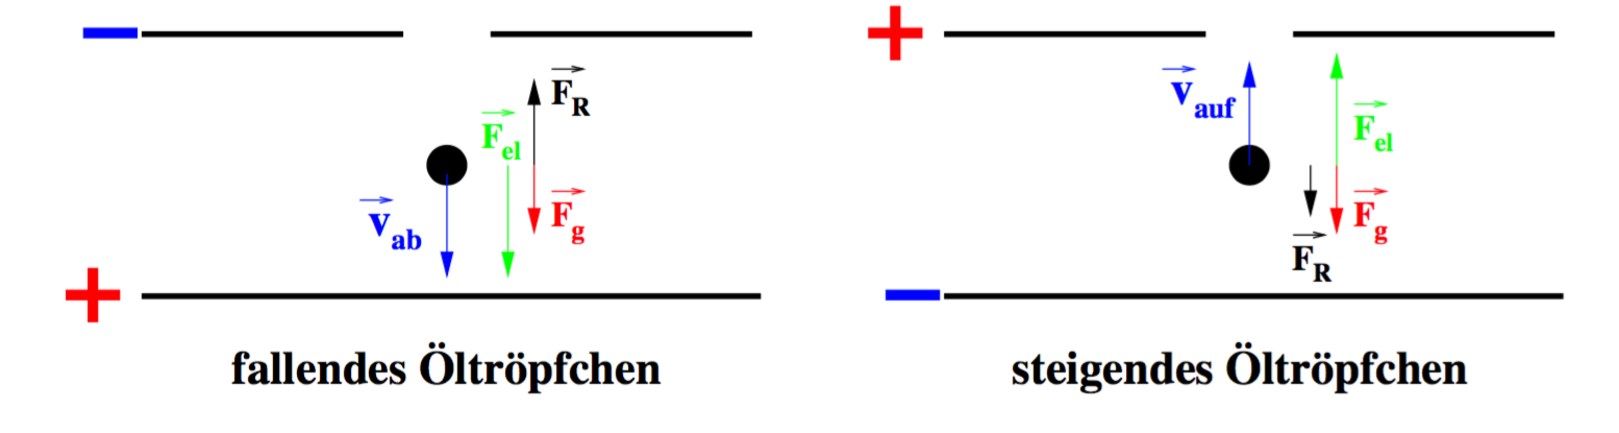
\includegraphics[width = \textwidth]{PicturePerfect/troepfchenimefeld.pdf}
  \caption{Kräfte auf einen geladenen Tropfen im homogenen elektrischen Feld.\cite{anleitung}}
  \label{fig:troepfchenimefeld}
\end{figure}
Wenn die elektrische Kraft $\vec{F}_\text{el}$ nach unten gerichtet ist, führt sie gemeinsam mit
der Gewichtskraft zu einer Bewegung nach unten mit der Geschwindigkeit $v_\text{ab} > v_0$. Dem entgegengestzt sind die
Reibungskraft und der Auftrieb. Damit ergibt sich Gleichung \eqref{eqn:efeldab}.
\begin{equation}
  \underbrace{\frac{4\pi}{3} r^3 (\rho_\text{Oel}-\rho_\text{L})g}_\text{Gewichtskraft und Auftrieb}
  - \underbrace{6 \pi \eta_\text{L} r v_\text{ab}}_\text{Reibungskraft}
  = \underbrace{-q E}_\text{elektrostatische Kraft}
  \label{eqn:efeldab}
\end{equation}

Bei nach oben gerichteter elektrischer Kraft bewegt sich das Tröpfchen mit einer betragsmäßig kleineren
Geschwindigkeit nach oben, da die Gewichtskraft und die Reibungskraft der Bewegung entgegengesetzt sind.
\begin{equation}
  \underbrace{\frac{4\pi}{3} r^3 (\rho_\text{Oel}+\rho_\text{L})g}_\text{Gewichtskraft und Auftrieb}
  + \underbrace{6 \pi \eta_\text{L} r v_\text{auf}}_\text{Reibungskraft}
  = \underbrace{+ q E}_\text{elektrostatische Kraft}
  \label{eqn:efeldauf}
\end{equation}
Die Geschwindigkeit heißt $v_\text{auf}$.

Aus Gleichung \eqref{eqn:efeldab} und \eqref{eqn:efeldauf} folgt für die Ladung
des Tropfens $q$:
\begin{equation}
  q = 3 \pi \eta_\g{L} \sqrt{\frac{9}{4}\frac{\eta_\g{L}}{g}\frac{(v_\text{ab}-v_\text{auf})}{(\rho_\text{Oel}-\rho_\text{L})}}
  \cdot \frac{(v_\text{ab} + v_\text{auf}}{E}
  \label{eqn:ladung}
\end{equation}
und für den Radius:
\begin{equation}
  r = \sqrt{\frac{9 \eta_\text{L} (v_\text{ab}-v_\text{auf})}{4 g (\rho_\text{Oel}-\rho_\text{L})}}.
\end{equation}

Da das Tröpfchen größere Abmessungen hat als die mittlere
freie Weglänge in der Luft $\bar{l}$ wird die Ladung korrigiert.
% \begin{equation}
%   \eta_\text{eff} = \eta_\g{L} \left(\frac{1}{1 + A\frac{1}{r}} \right)
%   = \eta_\g{L} \left(\frac{1}{1 + B\frac{1}{p r}} \right).
% \end{equation}
% Dieser Term heißt Cunningham-Korrekturterm mit $B = \SI{6.17e-3}{\text{Torr}\centi\meter}$.
Für die Ladung gilt dann:
\begin{equation}
  q = q_0 \left( 1 + \frac{B}{p_0 r} \right)^{\frac{3}{2}},
\end{equation}
wobei $B = \SI{6.17e-5}{\meter} \cdot \frac{p_0}{760}$.
